%!TEX root = ../xesphVII.tex
\chapter{稳恒电流}


\section{稳恒电流描述与形成}
\subsection{德鲁德模型}
电荷的定向移动形成\emph{电流}(current).\,就好像一缸气体在慢慢挪动那样,\,电荷的定向移动并不是纯粹的匀速运动,\,而是与无规则的热运动相叠加.\,1900年前后德鲁德({\it P. Drude})和洛伦兹({\it H. A. Lorentz})等人提出\emph{德鲁德模型}(Drude model)来解释金属中的导电现象.\,主要观点是金属内部自由运动的电子类似于理想气体那样做自由的运动,\,称为\emph{自由电子气}(free electron gas).\,我们用电子电量$-e$,\,质量$m$,\,电子数密度$n$,\,和\emph{弛豫时间}(relaxation time)$\tau$,\,平均速度$v$来表示其特征.\,弛豫时间就是电子做匀速直线运动,\,与原子实两次碰撞之间的平均间隔时间.\,与之相关的另一个量还可以是\emph{平均自由程}(mean free path)$\lambda$.\,容易想像,\,典型的情形是,\,常温下电子的平均速度是和气体分子的平均热运动速度那样,\,一个非常巨大的速度,\,而金属原子之间的距离又是那么地短,\,导致电子发生十分频繁的碰撞.\,而如果在金属中加一个电场$\bs{E}$,\,它在两次碰撞内是只可以让电子速度改变一个十分微小的量的:
\[\bs{a}=-\frac{e\bs{E}}{m}\]
\[\bs{v}(0)\quad\longrightarrow\quad\bs{v}(t)=\bs{v}(0)+\bs{a}t\quad\longrightarrow\quad\bs{v}(\tau)=\bs{v}(0)+\bs{a}\tau\]

我们根据统计力学的思想,\,计算在某一时刻电子速度对所有电子取热平衡分布的平均:
\[\bs{u}=\langle\bs{v}\rangle=\langle\bs{v}(0) +\bs{a}t\rangle = \bs{a}\tau\]

上式$t$代表距离上次碰撞每个电子幸存的时间.\,$\bs{v}(0)$代表上次碰撞后其速度.\,一方面,\,认为碰撞使得电子速度完全随机分布,\,平均的结果为零.\,另一方面,\,认为电子的碰撞是一个泊松过程,\,其碰后幸存时间的概率分布是一个指数分布:
\[p(t)=\ue^{-\frac{t}{\tau}}\]

从而平均的$t$为
\[\langle t\rangle=-\int_0^\infty t\ud p=\left. pt\right|^0_\infty+\int_0^\infty \ue^{-\frac{t}{\tau}} \ud t=\tau\]

最后结合电流密度为:
\[\bs{j}=-ne\bs{v}\]

我们得到:
\[\bs{j}=\frac{ne^2 \tau}{m}\bs{E}\]

的结果.\,称为\emph{微观欧姆定律}(microscopic Ohm's law),\,其中系数被称为\emph{电导率}(electrical conductivity):
\[\sigma=\frac{ne^2 \tau}{m}\quad;\quad \bs{j}=\sigma\bs{E}\]

十分值得指出的是,\,作为德鲁德模型的另一个重要结论,\,金属的\emph{热导率}(thermal conductivity)在理论中也可以给出一个估计值.\,我们都知道金属比绝大多数其他固体都拥有好得多的导热性能.\,这可以用热导率与\emph{傅里叶热传导定律}(Fourier's law of thermal conduction)来描述:
\[\bs{q}=-\kappa \nabla T\]

其中$\bs{q}$为热流密度,\,$\kappa$即为材料的热导率.\,水常温下热导率只有$0.591 \rm W/(m\cdot K)$,\,但纯的铜却能够达到$401 \rm W/(m\cdot K)$.\,金属的高热导率全都得益于轻盈的电子气,\,它能够迅速地把局部的热运动加剧传导开来.\,类比理想气体的非平衡态统计方法,\,我们给出:
\[\kappa=\frac{1}{3}nv\lambda c\]

式中$c$为每个电子的动能与温度的比.\,利用$\lambda=v\tau$,\,我们把热导率和电导率做比,\,便可以把较难确定的散射弛豫时间消去,\,得到:
\[\frac{\kappa}{\sigma}=\frac{mv^2c}{3e^2}\]

德鲁德模型认为,\,作为类似于理想气体的电子气,\,理应有:
\[c=\frac{3}{2}k\quad ;\quad \frac{1}{2}mv^2=\frac{3}{2}kT \]

从而得到:
\[\frac{\kappa}{\sigma T}=\frac{3}{2}(\frac{k}{e})^2\]

历史上金属热导率和电导率的比值与温度相关的现象很早就被人们发现,\,一般温度升高时电导率会有十分明显的下降,\,也就是金属的电阻会上升.\,小灯泡在未发光时与正常发光时电阻就经常有2倍左右的差距.\,而1853年魏德曼({\it G. Wiedemann})和弗朗茨({\it R. Franz})观察到不同金属虽然导电导热性能差距悬殊,\,室温下两者之比却接近一个常数,\,称为\emph{魏德曼-弗朗茨定律}(Wiedemann-Franz's law).\,而洛伦茨({\it L. Lorenz})\footnote{注意,\,丹麦物理学家路德维希·洛伦茨({\it Ludvig Lorenz})(1829-1891)与荷兰物理学家亨德里克·洛伦兹({\it Hendrik Lorentz})(1853-1928)是两个不同的人.\,有一个方程以它们两人的名字共同命名:\,Lorenz-Lorentz关系.}在1872则把这一经验规律确定到常数与绝对温度成正比的形式.\,最后德鲁德电子论将这个常数以微观常数的形式确定下来,\,等式右边现在约为$1.11\pow{8} \rm W \cdot\Omega /K^2$,\,这与实验结果数量级是一致的,\,但却差了约2倍.\,真实的值被称为\emph{洛伦兹常数}(Lorentz number):
\[\frac{\kappa}{\sigma T}=L=\frac{\pi^2}{3}(\frac{k}{e})^2=2.44\pow{8} \rm W \cdot\Omega /K^2\]

这个理论很成功,\,但最后的结果的不符合让人感到疑惑.\,还有一个令人感到疑惑的问题.\,就是对于电子气的电容.\,既然电子是完全独立于金属原子实的另一个热力学体系.\,按照经典统计物理.\,原子实的摩尔热容与离子晶体等类似,\,大概在$3R$附近\footnote{即\emph{督龙-裴替定律}(Dulong-Petit Law).}.\,而电子按只有平动自由度的理想气体考虑应贡献$1.5R$热容.\,实验却否定了这一点,\,金属常温下热容仍然是在$3R$附近.\,电子仿佛没有被热激发,\,然而电子又势必参与导热,\,因为金属的导热性能明显优于其他物质.\,那么以上推导过程中哪儿存在不合理之处?\,几年后到来的量子力学革命让人们认识到这一个经典模型从一开始就做了不止一个的与微观实际情况不符的假定,\,但又是十分巧合地,\,最终结果与真实值数量级自动一样了.

\subsection{费米气观点*}

元素周期律引发了人们对原子核外电子排布规律的研究,\,人们惊奇地发现电子是\emph{费米子}(fermion),\,符合\emph{泡利不相容原理}(Pauli exclusion principle).\,这赋予电子独特的量子特性.\,具体来说,\,单位体积内如果电子数目越多,\,那么其最低平均能量就必须越大.\,因为能量最低的状态一旦被占据,\,其他电子就必须占据能量更高的状态,\,即使按照最低能量的方式去堆积(绝对零度时的行为),\,电子也将具有很高的平均能量.\,它符合类似位置-动量不确定性原理的反比率,\,电子浓度的减小了单电子占据的位置尺度,\,则它的动量就会增加,\,从而根据色散关系$p^2=2mE$其能量也会升高.\,这一点使得我们去修改经典的德鲁德模型.\,相应的量子气体称为\emph{费米气}(Fermi gas).

定量计算费米气的特性需要考虑电子的波动本性.\,我们暂时取金属为长宽高为$ABC$的长方体,\,那么如果将$N$个电子倒入这个容器,\,电子的数密度为:
\[n=\frac{N}{ABC}\]

让我们考虑一下电子对状态的填充,\,长方体相当于一个谐振腔,\,事实上给出了电子动量状态的量子化:
\[p_x A=ah\;,\; p_y B=bh\;,\; p_z C=ch\]
\[a,b,c\in\mathbb{N}\]

这是因为根据德布罗意关系$p=\hbar k$而电子状态需要满足$kL=2m\pi$的缘故.\,从而我们发现电子的三个方向的动量都是量子化的.\,量子化的单位为:
\[\Delta p_x=\frac{h}{A}\;,\;\Delta p_y=\frac{h}{B}\;,\;\Delta p_z=\frac{h}{C}\]

\begin{wrapfigure}[16]{o}[-10pt]{7cm}
\centering
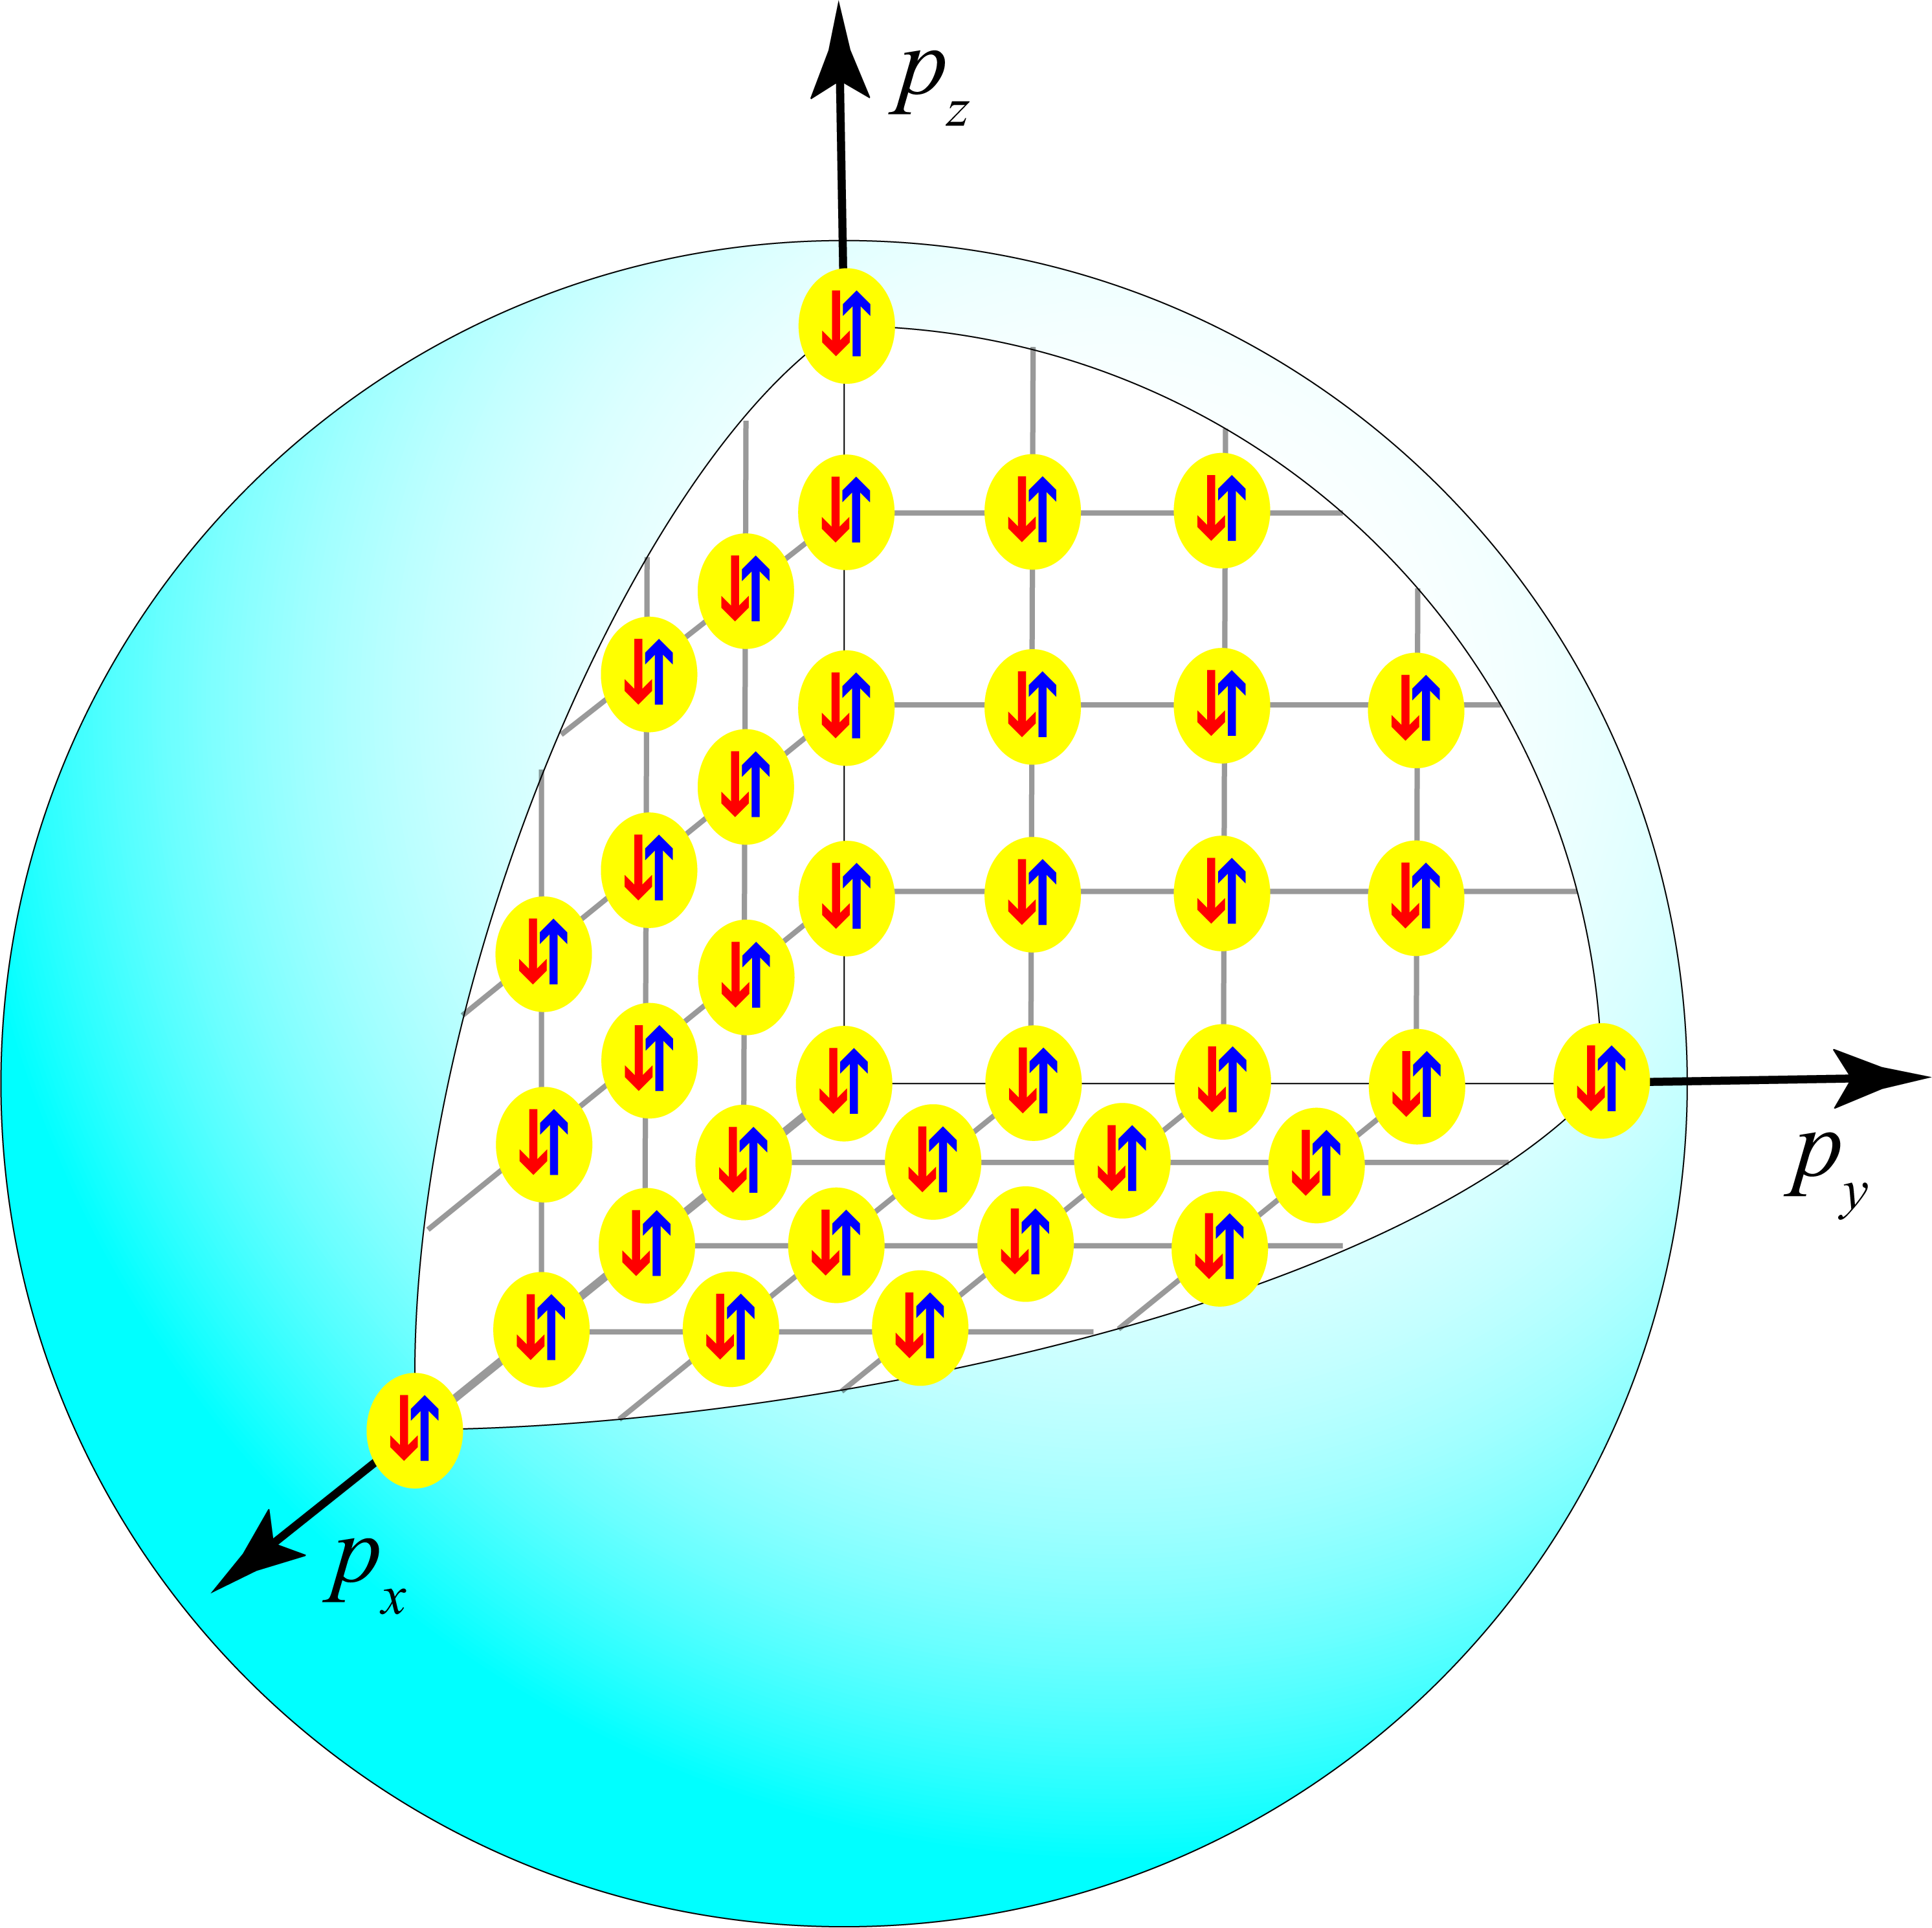
\includegraphics[width=7cm]{image/7-3-1.png}
\caption{电子态密度}
\end{wrapfigure}
现在把$N$个电子倒入动量空间中,\,那么电子在低温下将从最低能量态开始填充,\,由于电子数目巨大,\,最后电子将填充到能量为$\varepsilon_F$处.\,这样的一个填满电子的动量空间中的球体称为\emph{费米海}(fermi sea),\,最终填充到的能量称为费米能级$\varepsilon_F$,\,对应的电子动量为费米动量$p_F$.\,注意到一个动量空间中的一个标志状态的坐标内部实际上有两个独立的态,\,它们表示即使这两个波的波矢$\bs{k}$一样,\,它们代表电子的自旋也不一样\footnote{电子的微观描述是旋量波,\,也就是二分量波函数,\,具有两种可能的自旋.}.\,从而我们写出:
\[2\cdot\left.\frac{4\pi p_F^3}{3}\right/(\Delta p_x \Delta p_y \Delta p_z)=N\]

从而得到:
\[p_F=(\frac{3Nh^3}{8\pi N})^{\frac{1}{3}}=(\frac{3nh^3}{8\pi})^{\frac{1}{3}}\]

在以上过程中总电子数和总体积被消去了,\,最后电子堆积到的动量值仅仅取决于各处电子的数密度而成为了强度量.\,这样一个由于泡利不相容原理所造成的动量值对应到速度上,\,对一般金属估计约为$10^6\rm m/s$.\,而如果按非费米气计算,\,热运动速度应为$\sqrt{kT/m}\sim 7\pow{4}\rm m/s$,\,我们发现经典结果是严重估计少了的.\,但电子的热容又估计多了.\,量子统计给出:
\[c=\frac{\pi^2}{2}k\cdot\frac{kT}{\varepsilon_F}\]

代入热导率公式,\,得:
\[\frac{\kappa}{\sigma}=\frac{\pi^2}{6}\cdot\frac{mv_F^2}{\varepsilon_F}\cdot(\frac{k}{e})^2\cdot T\]

恰好,\,$\varepsilon_F=\dfrac{1}{2}mv_F^2$,\,从而我们得到了正确形式的魏德曼-弗朗茨定律:
\[\frac{\kappa}{\sigma T}=\frac{\pi^2}{3}(\frac{k}{e})^2\]

我们最后做一个经典德鲁德模型与量子费米气模型的比较.\,两个理论都承认以下基本公式的成立:
\[\sigma=\frac{ne^2 \tau}{m}\quad ,\quad \kappa=\frac{1}{3}nv^2\tau c\]

先看电导率,\,经典理论与量子理论对各个参数的估计除了$\tau$其他都是一致的.\,而经典更倾向于对$\tau$的估计更小.\,因为经典理论一般认为$\tau=\lambda/v$,\,而$\lambda$一般就按照原子实之间的平均距离来估计.\,这一点之后就知道是不妥当的,\,因为电子实际上可以在严格周期性的势能场中毫无散射的传播下去.\,而使得电子能够被散射的其实是晶格的缺陷,\,热振动等因素,\,从而一般温度升高,\,$\tau$减小,\,金属的导电性能就大大减弱.\,这给出了金属电阻随温度升高而升高的结论.\,这里经典理论对$\lambda$的过低估计恰好被对$v$的过低估计所抵消掉一部分,\,从而最后$\tau$的值在常温下差距也不大.\,而对于热导率,\,经典理论对$v$的过低估计又恰好被对$c$的过高估计修正,\,精确到了仅仅相差一个常数,\,除了经典理论说不清楚的$\tau$,\,经典与量子的在数量级上是基本符合的.

值得一提,\,热导率描述导热,\,电导率描述导电,\,而导电现象的附效应便是热产生.\,也就是\emph{焦耳热}(Joule heating).\,微观的功率密度
\[\bs{j}=\sigma \bs{E}\quad ,\quad w=\bs{j}\cdot\bs{E}\]

也即:
\[w=\sigma \bs{E}^2=\rho \bs{j}^2\]

其中\emph{电阻率}(resistivity)$\rho$为电导率的倒数.\,上为\emph{微观焦耳-楞次定律}(microscopic Joule-Lenz law).

\subsection{能带论*}

费米气模型在量子力学迅猛发展的几十年后回头看又是过于na\"\i ve了.\,人们发现电子终究是在晶格间传播的波动,\,如果原子实与背景的电子给出了严格的周期性的势能,\,那么如果电子的总机械能小于最大势能,\,那么就成为了束缚态,\,限制在一个原子附近运动而成为原子实的一部分.\,而如果电子守恒机械能大于最大势能,\,就成为不受任何阻碍的传导态.\,动能虽在运动中有所波动,\,但绝不会越来越小.\,描述电子的波函数称为\emph{布洛赫波函数}(Bloch wave function).\,而电子如何去填充怎样的能级?\,\emph{布洛赫}({\it F. Bloch})研究并发现了\emph{能带论}(energy band theory)来替代旧的费米气理论,\,这个理论可以统一地描述导体与绝缘体.

能带论可以看成是电子在单原子外的束缚态特征与传导的自由电子气的特征的一种综合,\,一方面电子在这样的一个周期性势场中的运动其守恒的机械能并不是可以取所有值,\,而是分为可以连续取值的区间:\,\emph{能带}(band)与根本取不到的能量区间:\,\emph{带隙}(gap)所构成.\,而电子作为波动用其所在的能带与波矢$\bs{k}$来描述.\,其波矢方向的物理意义不再重要,\,因为每一个态一般都代表某种驻波与行波的混合,\,而每一个态附近的群速度则可以代表这个态代表的真实电子运动速度.\,另一方面这些能带的结构又恰好对应到了单原子的束缚态能级.\,这使得我们经常是一望某元素的单原子核外电子排布,\,便能从其是否具有最外层电子读出这种元素单质是否能导电的信息.
\begin{figure}[H]
\centering
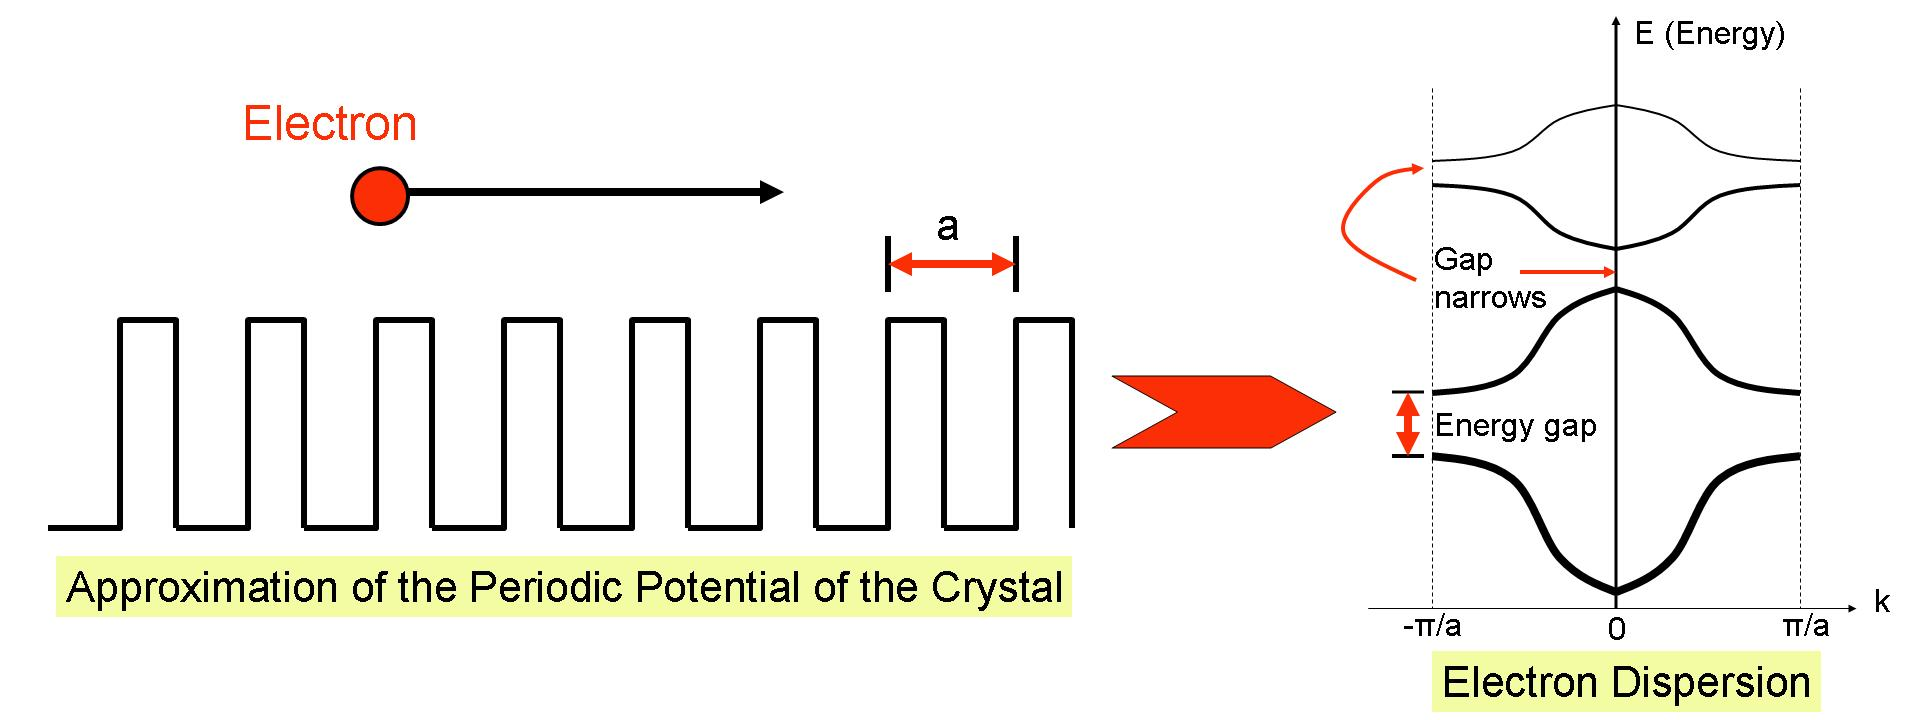
\includegraphics[width=0.8\textwidth]{image/7-3-2.jpg}
\caption{电子在周期性势场中传播}
\end{figure}

某种原子形成晶体时,\,电子从最低的能带开始填充,\,内层电子填满了较低的那些能带,\,它们不参与导电,\,对应于原子实电子和在晶体共价键键合的价电子.\,最外层电子较少的原子,\,形成晶体时最后填充的那个能带没有填满,\,或者虽然填满但与下一个能带在能量区间上重合而能够导电.\,称为\emph{导体}(conductor).\,对应的元素也就显示出明显的金属性\footnote{思考:\,氢是否具有金属性?\,参考\url{https://en.wikipedia.org/wiki/Metallic_hydrogen}.}.\,而若原子外层电子数目多,\,则很有可能电子恰好填满一个能带后隔着一个能隙与空的上方能带相望,\,则所有态都稳定不变,\,材料所有电子都是束缚电子,\,最后填充的那个满带称为\emph{价带}(valence band),\,代表原子间成共价键的价电子所在的能带.\,而上方的那个空带称为\emph{导带}(conduction gap).\,意为一旦这个带中存在电子则会大大改善其导电性能.\,此时元素体现出非金属性,\,一般形成的都是\emph{绝缘体}(insulator).\,而在金属性元素与非金属元素分界处则存在很多的\emph{类金属}(metalloid),\,它们形成的晶体虽然与绝缘体一样,\,在最低能量时恰好把价带排满,\,而隔着一个带隙与空的导带相望.\,但带隙很小(小于$4{\rm eV}$),\,导致常温的热激发和掺杂,\,抑或是光照激发都将在导带中激发大量载流子而具有可观的导电性能.\,这些材料称为\emph{半导体}(semiconductor).
\begin{figure}[H]
\centering
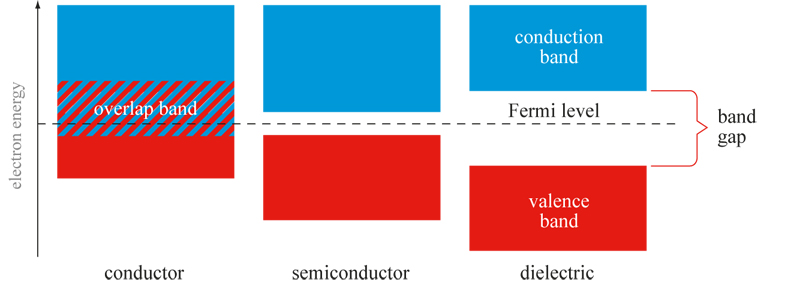
\includegraphics[width=0.8\textwidth]{image/7-3-3.jpg}
\caption{能带与导电性}
\end{figure}
\begin{figure}[H]
\centering
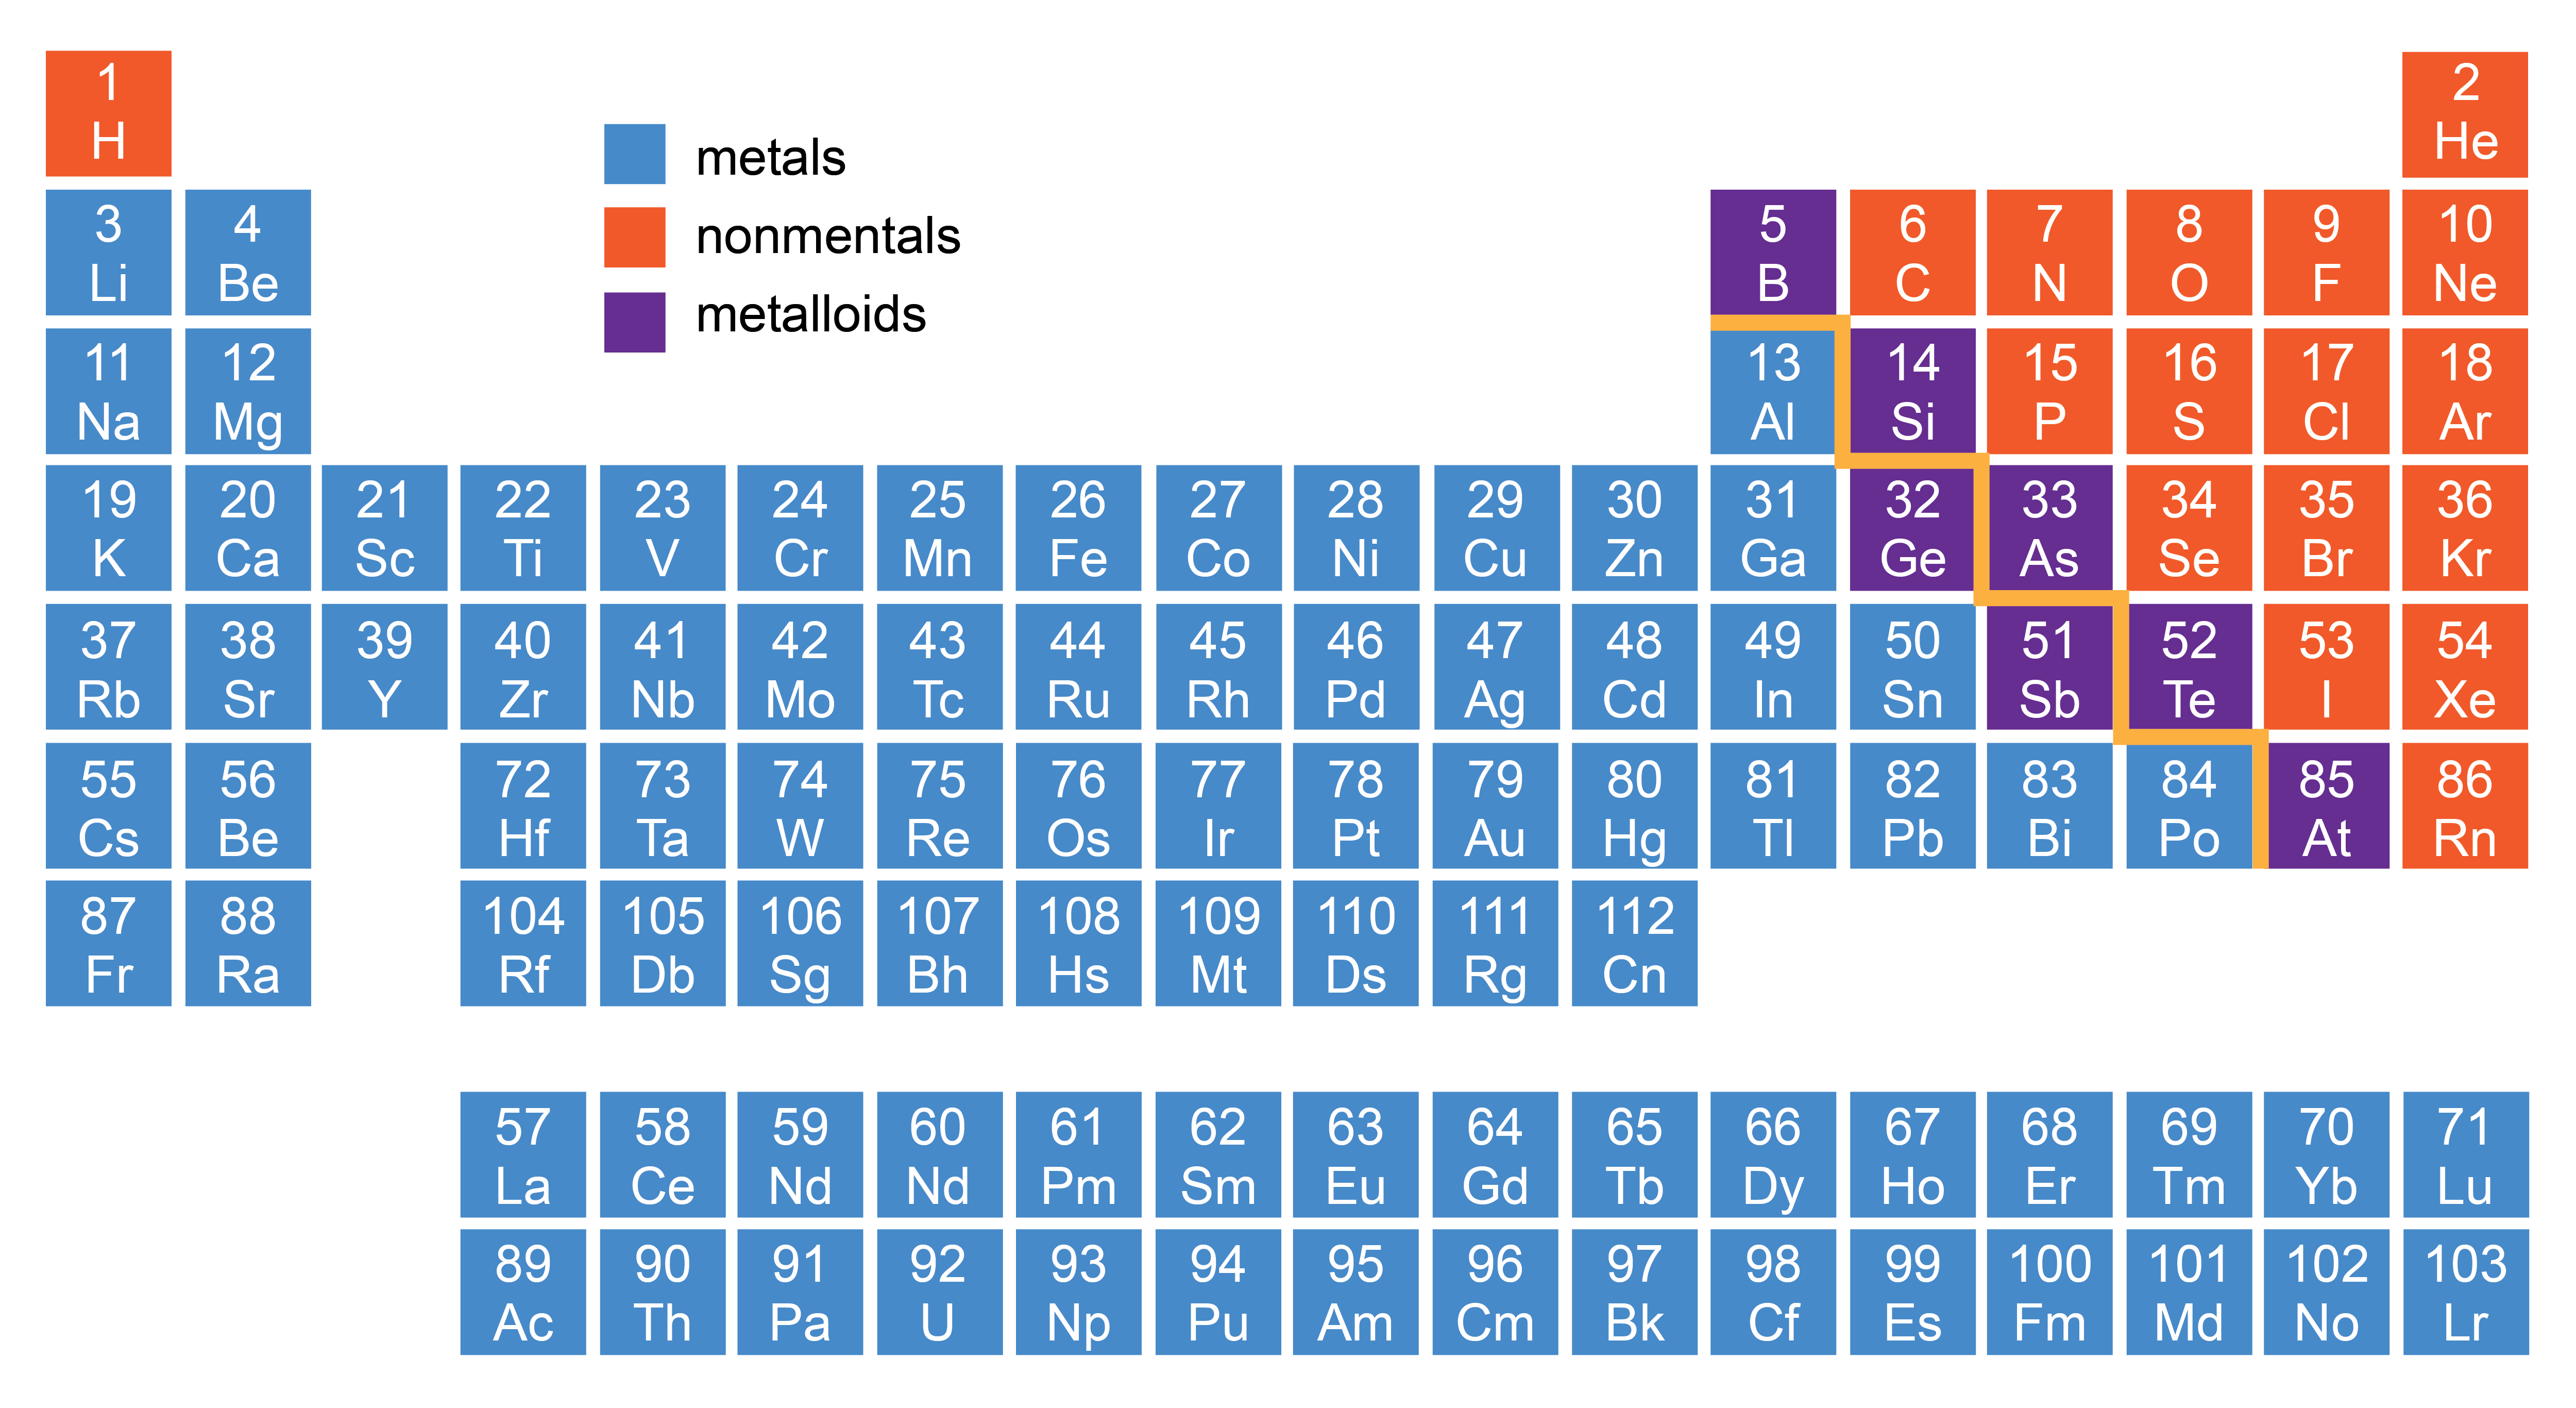
\includegraphics[width=0.8\textwidth]{image/7-3-4.jpg}
\caption{金属,\,类金属与非金属元素}
\end{figure}

那么能带论如何给出电导率的计算公式?\,仍然是:
\[\sigma=\frac{ne^2 \tau}{m}\]

与上一个费米气模型区别在于一点,\,就是这里的$m$不再是电子的\emph{裸质量}(bare mass),\,而是由于与周期性势场相互作用,\,电子的色散关系(能量与波矢关系)被修正后给出的\emph{有效质量}(effective mass).\,即使对于金属,\,这个质量与真实电子质量相差好几倍的现象也是十分普遍的.



\subsection{惯性,\,阻尼与回复力}

在量子力学还未诞生的时期,\,为了解释导体的导电,\,绝缘体的介电现象,\,并适用于任意交变电磁场在介质中的传播,\,色散,\,吸收与散射.\,洛伦兹提出著名的\emph{洛伦兹模型}(Lorentz model)作为德鲁德模型的补充.\,在这儿电子的惯性被重视,\,电子与晶格的碰撞被简化,\,可能的原子实对电荷的束缚被简化为线性回复你.\,也就是洛伦兹用唯象的谐振子类比来解释电子在外场下的行为:
\[m\ddot{\bs{r}}+\gamma \dot{\bs{r}}+ k\bs{r}=-e\bs{E}\ue^{i\omega t}\]

这个模型的解和它对应的各种特性我们将在光学教材里详细讲解.\,在这里我们仅仅讨论导体中的自由电子,\,故$k=0$.\,与导体导电相关的两个因素为:

一是阻尼系数$\gamma$.\,在直流电场下平衡时稳定的电子速度为:
\[\dot{\bs{r}}=-\frac{e}{\gamma}\bs{E}\]

对比更加本质的德鲁德等导电模型的电导公式,\,容易发现这个唯象系数与电导率和基本参量关系为:
\[\gamma=\frac{ne^2}{\sigma}=\frac{m}{\tau}\]

于是我们可以写出在导体上突然加一个不随时间变化的匀强电场后电子的运动的微分方程:
\[m\ddot{\bs{r}}+\frac{m}{\tau} \dot{\bs{r}}=-e\bs{E}\]

它的解为:
\[\dot{\bs{r}}=-\frac{e\bs{E}\tau}{m}(1-\ue^{-\frac{t}{\tau}})\]

我们十分自然地发现定义电子碰撞的弛豫时间恰好与导体对电场响应的弛豫时间相吻合.\,这一点稍微需要一些讨论和修正.\,见下.

第二点我们来讨论表示电子惯性的质量$m$.\,正是它导致了衰减因子$\ue^{-\gamma t/m}$,\,从而造成电路对电场响应的弛豫.\,但如果讨论电路的弛豫,\,或者说电流的惯性,\,有一点是被我们过低地估计了,\,便是自感现象.\,电荷的加速运动形成变化的电流,\,从而与之相伴的是变化的磁场.\,这个变化的磁场反过来给电流一个反向的作用力.\,由于该力正比于加速度,\,故等价于增加了载流子的质量.\,这里的弛豫时间对应直流暂态电路中的$\tau^\prime=L/R$.\,如果一定要理解为电子的惯性质量,\,那么一般比电子的裸质量要大好几个数量级$m^\ast\gg m$.\,从而一般有电路弛豫时间$\tau=m^\ast/\gamma$不等于微观碰撞弛豫时间.

纯粹的导体是否有回复力项?\,显然在以上电子运动方程中不含这一项.\,但注意到如果有回复力项,\,即使外场为零电子也会做振动.\,真实情况会发生这样的现象吗?\,答案是会,\,即\emph{等离子体振荡}(plasma oscillation).\,原因是电子相对于原子实的位移实际上在金属的表面累积了电荷分布,\,从而在内部激发了电场.\,由于频率很高,\,一般要到紫外波段的频率,\,我们可以完全忽略阻尼的影响.\,当电子有位移$\bs{r}$时将形成极化强度\footnote{显然此时``极化强度''描述的非极化电荷,\,而是自由电荷.}:
\[\bs{P}=-ne\bs{r}\]

我们考虑块状金属板\footnote{的确,\,取不同形状的物体这个频率会有所不同.}的集体等离子体振荡,\,那么由于金属表面的累积电荷在金属内部形成的电场为:
\[\bs{E}=\bs{E}_{\rm in}=-\frac{\bs{P}}{\varepsilon_0}=\frac{ne\bs{r}}{\varepsilon_0}\]

代入原方程:
\[m^\ast \ddot{\bs{r}}=-e\bs{E}=-\frac{ne^2\bs{r}}{\varepsilon_0}\]

从而得到谐振子方程.\,振荡频率为:
\[\omega_p=\sqrt{\frac{ne^2}{\varepsilon_0 m^\ast}} \quad;\quad\sigma=\varepsilon_0\omega_p^2\tau\]

最后我们考虑低频电磁波(内部实际场强)下金属的电子行为,\,利用光学中讨论过的洛伦兹模型,\,我们计算金属的复电容率,\,最后得到:
\[\varepsilon_r(\omega)=1-\frac{\omega_p^2\tau^2}{1+\omega^2\tau^2} \quad ; \quad \sigma(\omega)=\frac{\sigma}{1+\omega^2\tau^2}\]

一般$\omega_p\tau\gg 1$,\,故低频下金属的介电常数实际上是绝对值很大的负数.\,电导率随着频率的增加而减小.


\subsection{稳恒电流与形成条件}

作为电荷的流动,\,电流密度与电荷密度间满足电荷守恒定律:
\[\nabla\cdot\bs{j}+\frac{\partial\rho}{\partial t}=0\]

而所谓\emph{稳恒电流}(steady current)指的是一定区域内导电物质形成的电荷,\,电场,\,电流分布.\,其中电流的分布不能随时间变化,\,自然的结论是电荷密度分布也不能随时间变化.\,否则将产生随时间变化的电场,\,电场造成电流的变化.\,即上式必有:
\[\frac{\partial\rho}{\partial t}=0\quad;\quad \nabla\cdot\bs{j}=0\]

即在稳恒电流中电流密度是一定没有散度的,\,无头无尾的闭合曲线.\,稳恒电流必须是\emph{直流}(direct current)而非\emph{交流}(alternating current).

容易发现,\,在稳恒电流中微观欧姆定律写成以下形式是不完整的:
\[\bs{j}=\sigma \bs{E}\]

在很多情况下,\,上式并没有问题.\,$\bs{E}$被理解为由电荷分布$\rho$形成的静电场\footnote{实际上,\,不包括涡旋电场,\,因为它被归于之后引入的非静电力.\,换句话说,\,这里的$\bs{E}$不再由静止电荷的受力$\bs{F}/q$去定义,\,而是单纯根据静止电荷分布产生平方反比的电场叠加去定义.},\,它是一定可以引入电势的:
\[\bs{E}=-\nabla\varphi\]

\begin{wrapfigure}[13]{o}[-10pt]{8cm}
\centering
\vspace{-0.3cm}
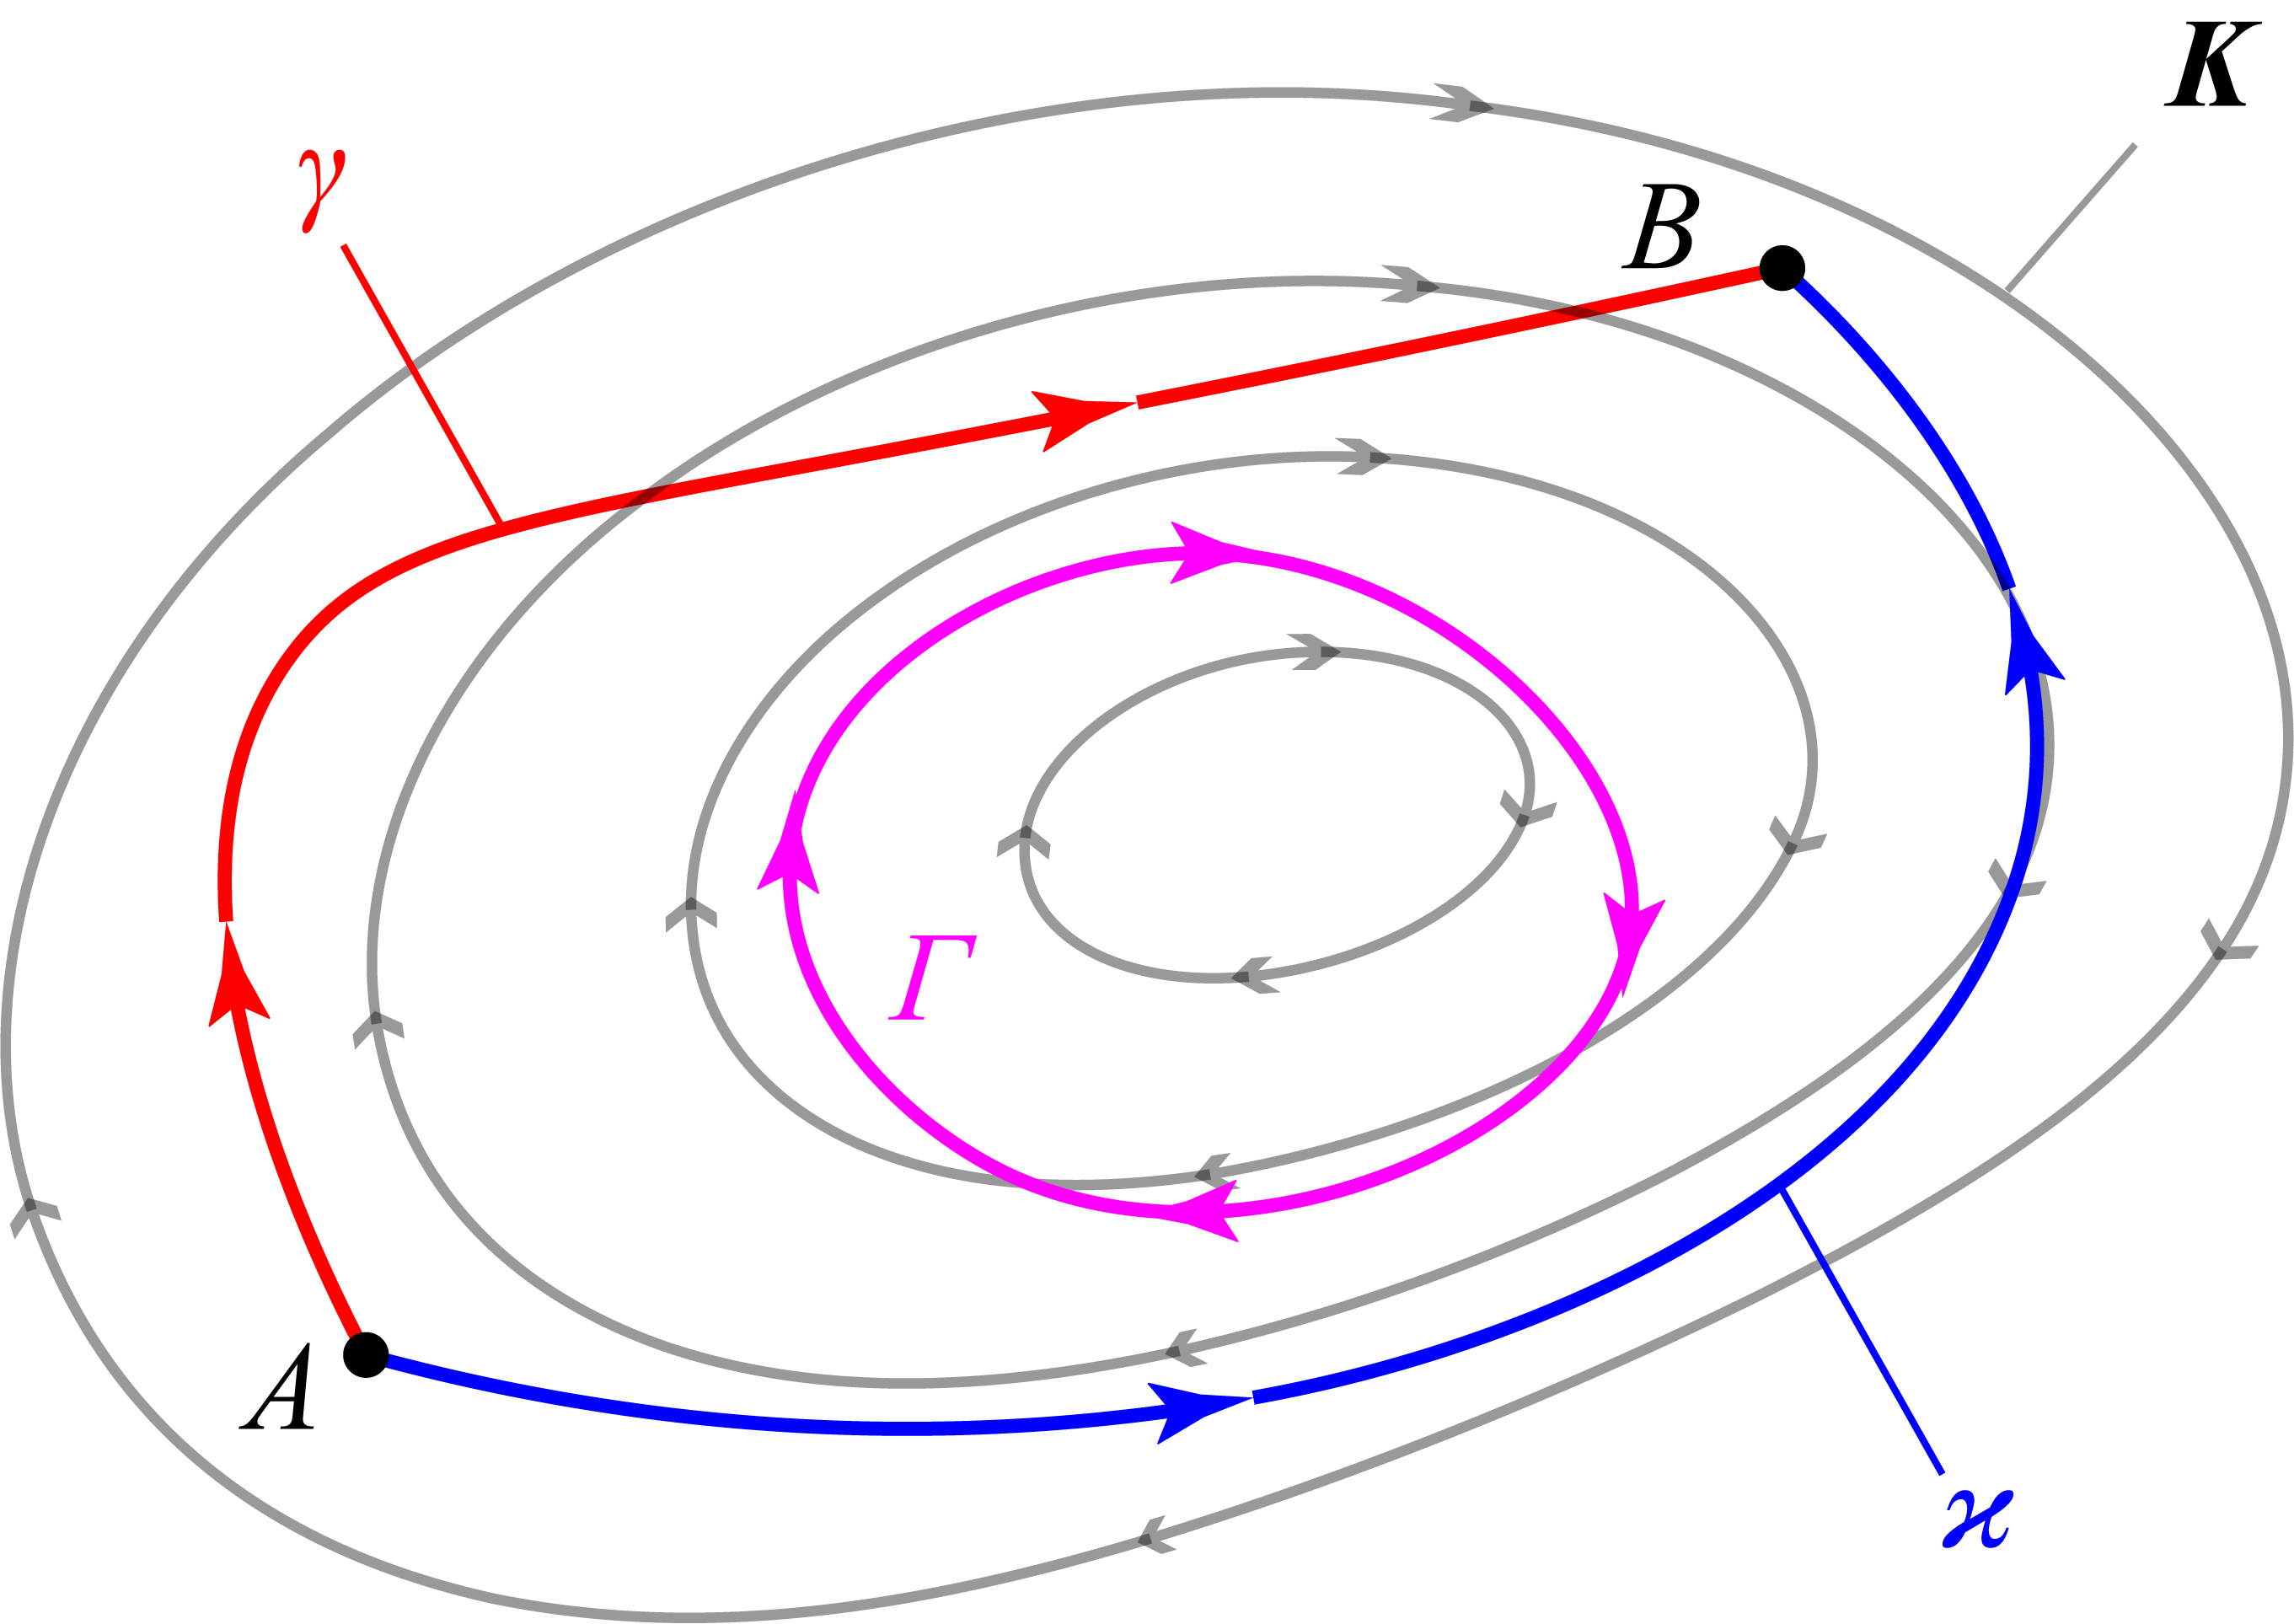
\includegraphics[width=8cm]{image/7-3-5.png}
\caption{非静电场}
\end{wrapfigure}
那么如果承认以上形式的微观欧姆定律就会引起矛盾:\,电流线是环状闭合的,\,电场线必须与电流线同向平行,\,但电场线又不能是闭合的,\,否则与静电场环路定理,\,电势的可定义性矛盾.\,实际上,\,微观形式的欧姆定律必须被写成:
\[\bs{j}=\sigma (\bs{E}+\bs{K})\]


上式$\bs{K}$代表\emph{非静电力场}(non-electrostatic field)对电子产生的作用.\,定义方式与电场量纲一致,\,都是单位正电荷的受力.\,这么写的不同之处就在于,\,把驱动电流的力分成了两部分:\,静电场$\bs{E}$是保守的,\,可以引入势的,\,在一个回路中不做功的,\,不吞吐能量的场(注意电流本身就会发热,\,这不是场造成的而是电荷定向流动碰撞晶格造成的).\,但非静电力就是源源不断做功驱动回路中电流流动的,\,非保守的,\,不能引入势来描述的场.\,虽然不能引入电势来描述非保守力,\,但可以用\emph{电动势}(electromotive force)来描述非静电力:
\[\mathscr{E}_\gamma=\int\limits_{A\stackrel{\gamma}{\longrightarrow}B} \bs{K}\cdot\ud\bs{r}\quad;\quad \mathscr{E}_\varGamma=\oint\limits_{\varGamma}\bs{K}\cdot\ud\bs{r}\]

不像对静电场的积分那样仅仅取决于端点,\,电动势与积分路径一一对应.\,回路电动势一般来说不为零,\,从而相同端点的两个路径电动势也不一定相等:
\[\mathscr{E}_\varGamma\neq 0\quad;\quad \mathscr{E}_\gamma\neq\mathscr{E}_\varkappa\]

非静电力既然能够作用在电子上,\,其形式一般就是电磁力,\,万有引力,\,或是惯性力.\,磁场力对应\emph{动生电动势}(motional emf),\,而由于变化的磁场激发的涡旋电场部分的电场力对应\emph{感生电动势}(transformer emf).\,电子会受到引力,\,1967年Schiff指出电子会因为引力的原因聚集到金属的底部.\,而后Dessler提出了严格的考虑晶格在重力场下压缩与不均匀情况下的电子平衡情况.\,引力是很弱的保守力,\,对金属内部电荷体系的影响虽然很小但绝不是不可观测.\,而与引力类似的惯性力则可以人工制造出很大的数值,\,而且可以使它非保守.\,试想加速旋转一个线圈,\,那么在随晶体加速的参考系里电子受到的角向惯性力就和受到一个电场力造成的效果没有本质的区别.

\begin{wrapfigure}[13]{o}[-10pt]{8cm}
\centering
\vspace{-0.5cm}
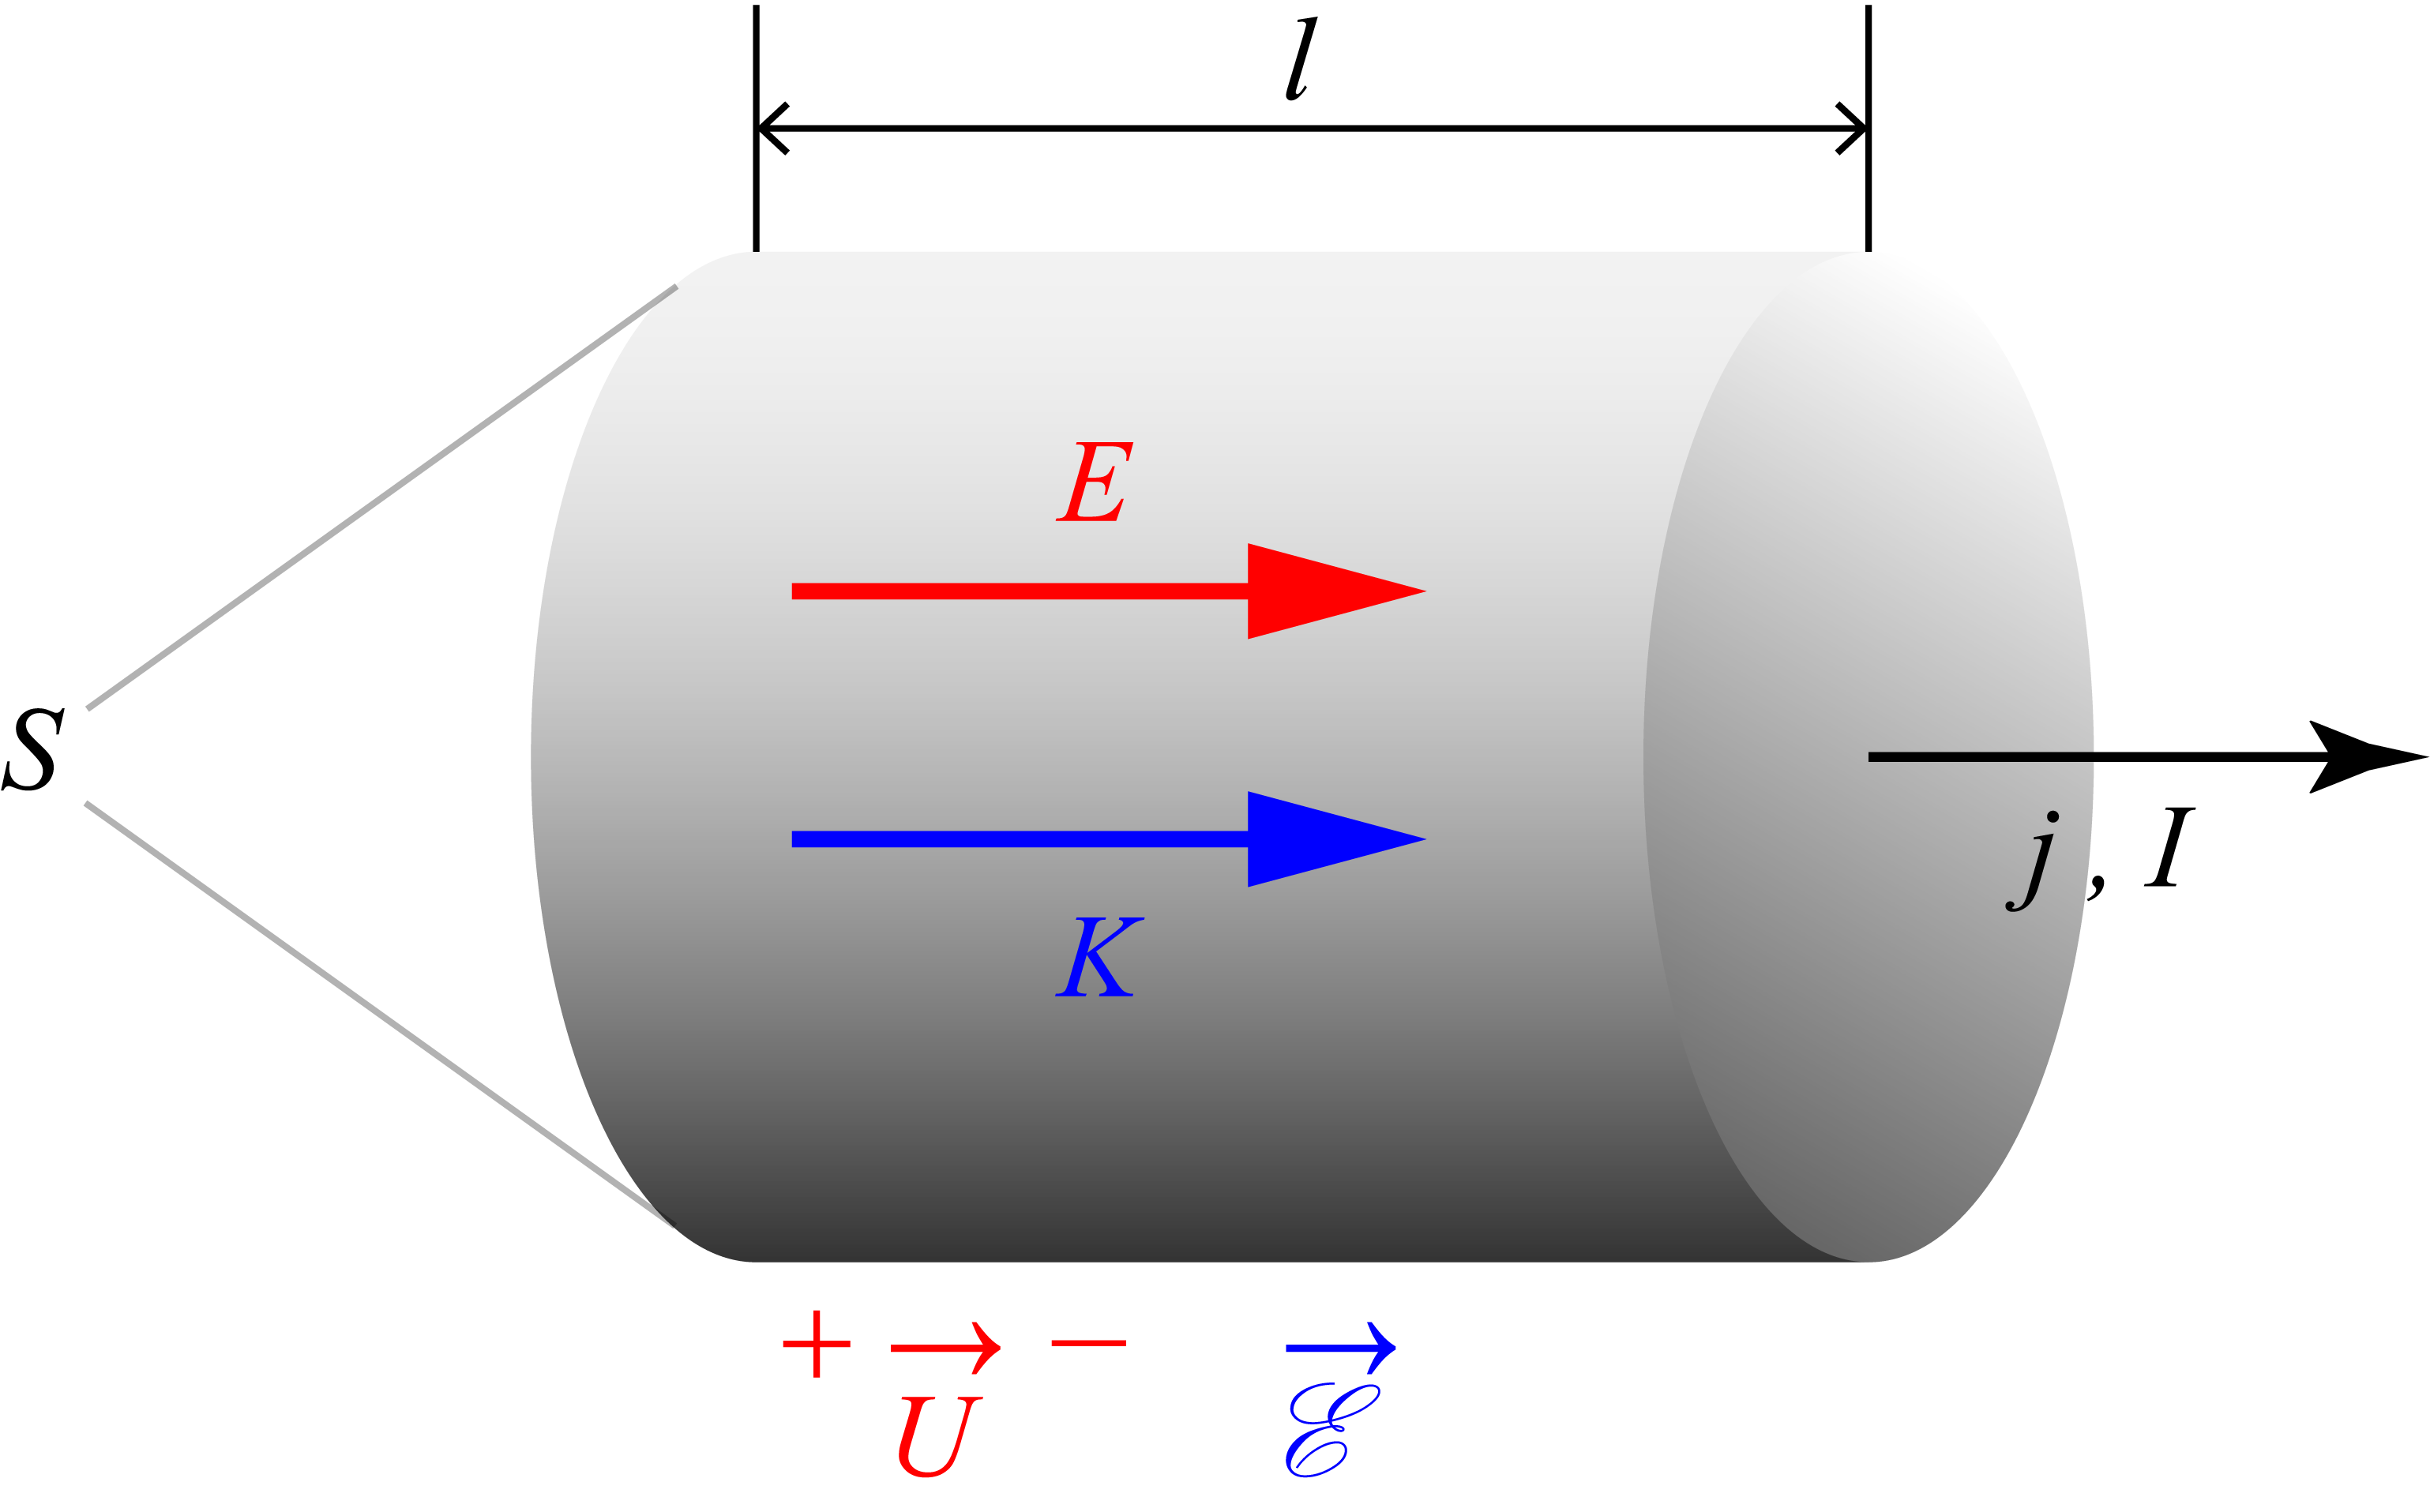
\includegraphics[width=8cm]{image/7-3-6.png}
\caption{宏观欧姆定律}
\end{wrapfigure}
还有一些电动势一般无法用非静电力描述.\,因为在一个回路中某些部分的确有能量的输入,\,但不是以作用在某些具体的电荷上的力的形式.\,而是更加广义的一些力作用在一些流上.\,例如温差电偶利用两种物质的电子的热扩散性质差异,\,从高温端吸取热量而驱动电流.\,化学反应更是源源不断地产生新的物质,\,利用反应的自发性而驱动物质做定向的移动形成电流.\,在这些抽象的场合,\,我们采用某段电路中移动单位电荷,\,外界向体系注入的能量来定义电动势:
\[\mathscr{E}=\frac{\ud W}{\ud Q}\]

\begin{figure}[H]
\centering
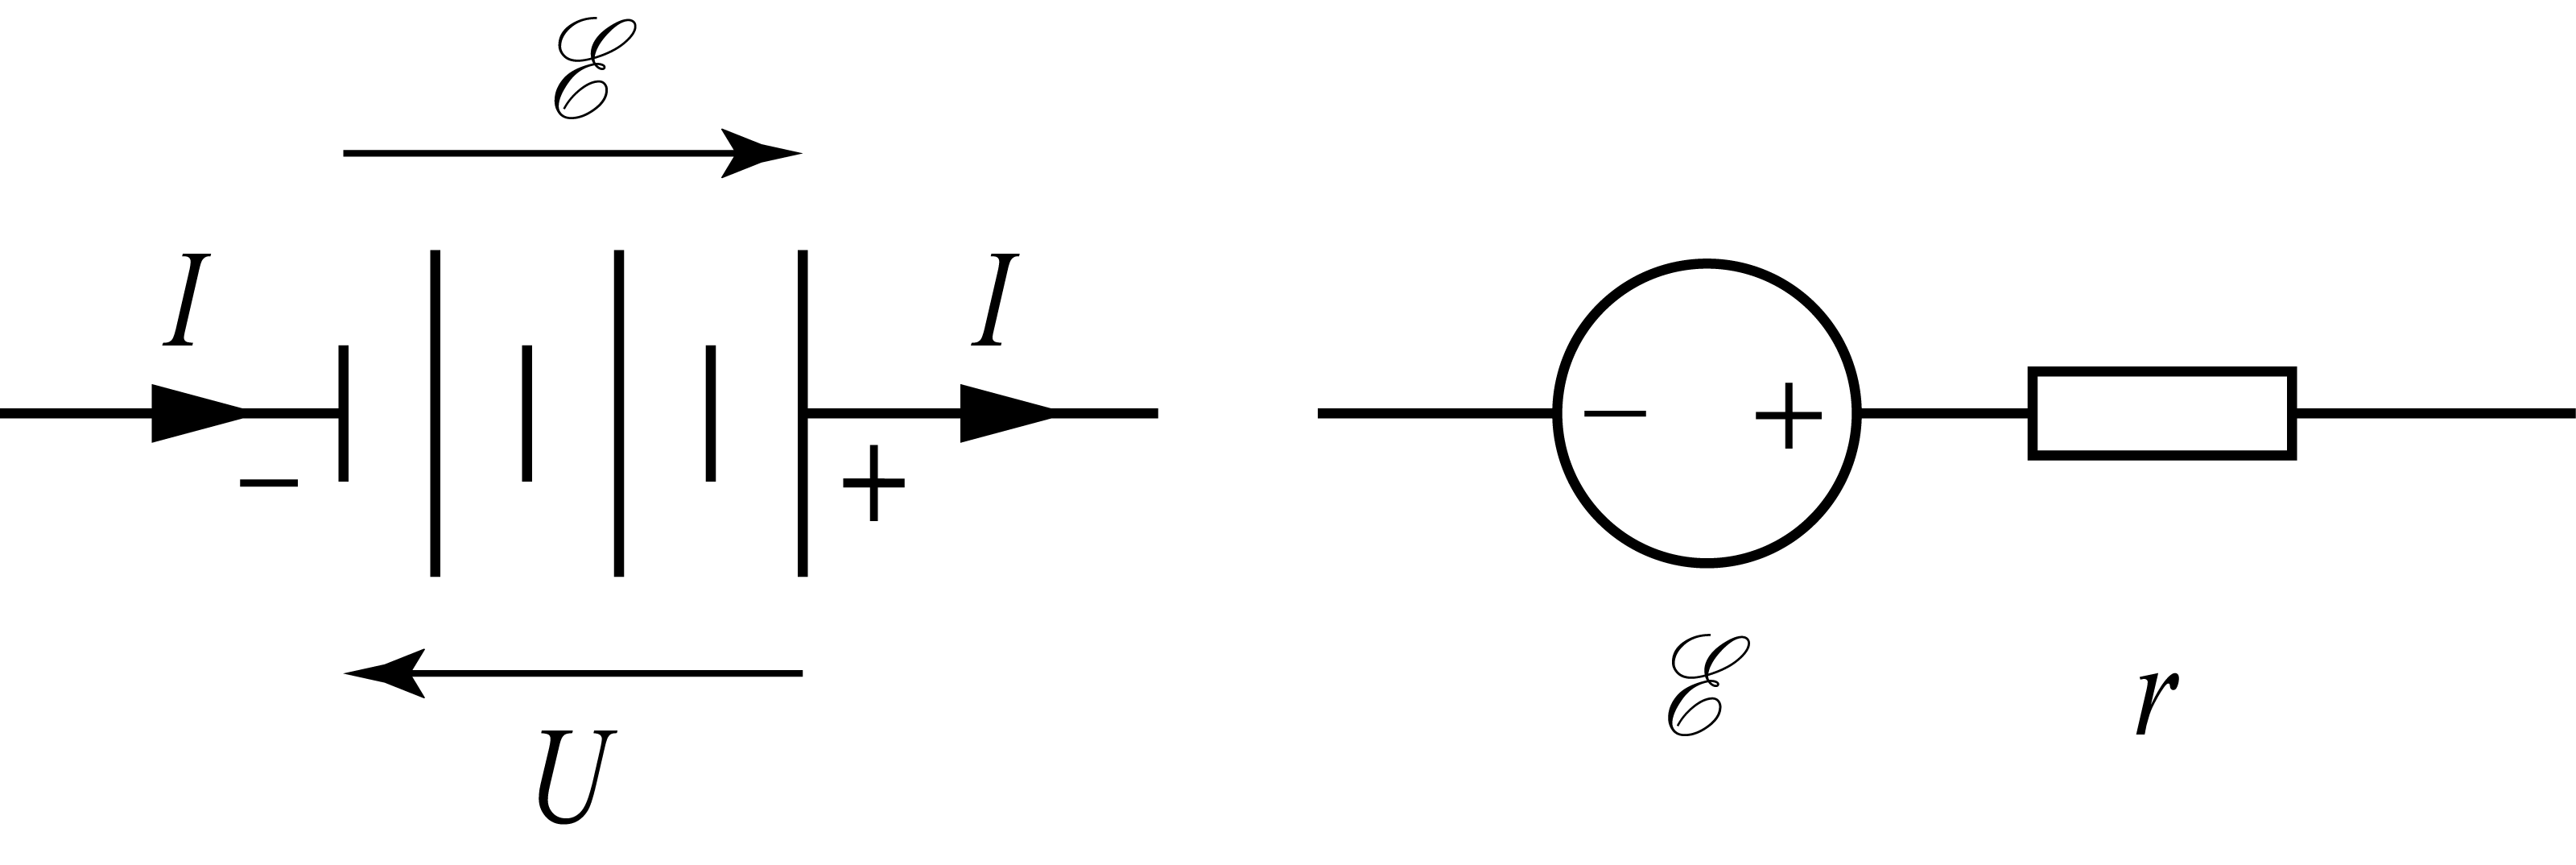
\includegraphics[width=0.6\textwidth]{image/7-3-7.png}
\caption{电池的欧姆定律}
\end{figure}
最后,\,从微观到宏观,\,我们考虑一段长为$l$,\,面积为$S$,\,电阻率为$\rho$的导体上的欧姆定律:
\[E+K=\rho j\]

等式两边同时乘以$l$,\,把电流密度写成$I/S$.\,得到:
\[U+\mathscr{E}=IR \quad;\quad R=\rho\frac{l}{S}\]

一般叫做部分电路的欧姆定律.\,而如果考虑\emph{电池}(battery)的两端,\,正常工作时一般正极电压更高,\,故约定电动势与电压取相反的方向,\,电流则与电动势方向一致,\,却与电压方向反向:
\[U=\mathscr{E}-Ir\]

为一段含源电路的欧姆定律.\,此时我们把电池等效为理想电压源和一个定值电阻$r$的串联.\,电阻即为电池的\emph{内阻}(internal resistance).






\section{电路与电路方程}

具体到直流电路中,\,我们一般提供以下理想的电路元件:

\section{电路分析基础}

\section{电路分析方法}

\section{半导体}
